\documentclass[tikz,border=5pt]{standalone}

\usepackage{amsmath} % for \text
\usepackage{xfrac} % for \myfrac
\usepackage{bm} % for \bm
\usetikzlibrary{calc}
\usetikzlibrary{positioning}
\usetikzlibrary{decorations.pathreplacing,decorations.markings}
\usetikzlibrary{patterns} % 加载 patterns 库
\usepackage{comment}

\usepackage{newtxtext,newtxmath} % 推荐LaTeX数学字体方案
\tikzset{every node/.style={font=\rmfamily}} % 所有节点都用罗马体

\usetikzlibrary{calc}


\colorlet{myred}{red!80!black}
\colorlet{myblue}{blue!80!black}
\colorlet{mygreen}{green!60!black}
\colorlet{myorange}{orange!70!red!60!black}
\colorlet{mydarkred}{red!30!black}
\colorlet{mydarkblue}{blue!40!black}
\colorlet{mydarkgreen}{green!30!black}
\colorlet{myred2}{red!50!white}

\colorlet{mylightblue}{blue!60!cyan!80!black!15}
\colorlet{mypurple}{blue!50!red!70}
\colorlet{gaugecol}{red!90!black!70} % Wiki red
\colorlet{leptoncol}{green!80!black!70} % Wiki green
\colorlet{quarkcol}{blue!85!cyan!95!black!55} % Wiki purple
\colorlet{quarkred}{red!98!black!55} % quark red
\colorlet{quarkblue}{blue!85!cyan!98!black!55} % quark blue
\colorlet{quarkgreen}{green!95!black!55} % quark green
\colorlet{gluoncyan}{cyan!100!black!55} % gluon cyan
\colorlet{gluongreen}{green!75!blue!95!black!70} % gluon green
\colorlet{gluonyellow}{yellow!98!black!55} % gluon yellow
\colorlet{gluonorange}{orange!100!black!65} % gluon orange
\colorlet{gluonmagenta}{magenta!100!black!70} % gluon magenta
\colorlet{scalarcol}{yellow!70!orange!98!black}
\colorlet{tensorcol}{blue!50!red!70} % Wiki light blue
\colorlet{groupcol}{orange!15}

\tikzset{
    mynode/.style={
        circle,        % 形状为圆形
        fill=black,    % 填充颜色为黑色
        inner sep=0.4, % 点的大小
        draw           % 添加边框
    }
}


\begin{document}

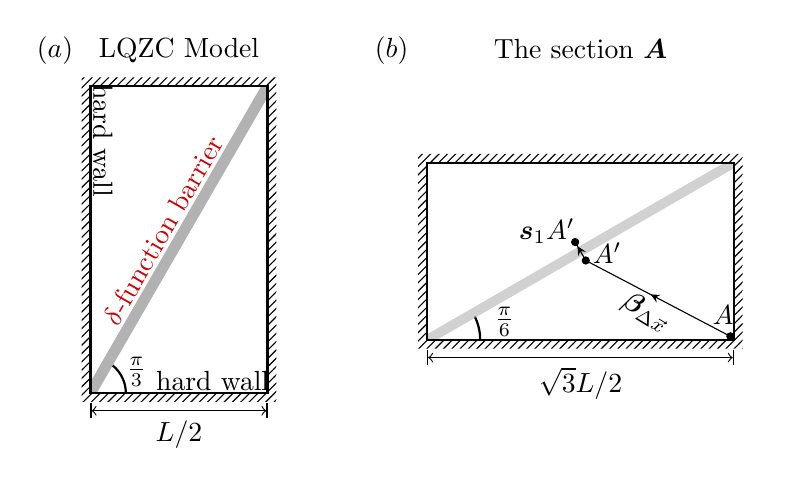
\begin{tikzpicture}[x=4.5cm, y=4.5cm]

\def\th{60}

\def\De{0.025}

% 定义点


\pgfmathsetmacro{\x}{cos(\th)}
\pgfmathsetmacro{\y}{sin(\th)}

\coordinate (PS) at (0, 0);


\coordinate (P1) at ($(0,0) + (PS)$);
\coordinate (P2) at ($(\x,0) + (PS)$);
\coordinate (P3) at ($(\x,\y) + (PS)$);
\coordinate (P4) at ($(0,\y) + (PS)$);
\coordinate (P5) at ($(\x/2,\y/2) + (PS)$);
\coordinate (PT) at ($(\x/2,\y + 0.1) + (PS)$);


\begin{scope}
\clip (0,0) rectangle (\x, \y);
\draw[thick] (0.1, 0) arc[start angle=0, end angle=60, radius=0.1];
\draw[gray!60, line width=4.0] (P3) -- (P1) node[midway, above, sloped, yshift = -2, color = myred] {$\delta$-function barrier};

\node[yshift = 4.4] at ($(P1)!0.69!(P2)$) {hard wall};
\node[rotate = 270, yshift = 4.5, xshift = -2.5] at ($(P4)!0.2!(P1)$) {hard wall};

\end{scope}

% 使用 even odd rule 填充“回”字形区域
    \fill[pattern=north east lines, even odd rule]
        (0-\De,0-\De) rectangle (\x+\De,\y+\De)   % 外矩形
        (0,0) rectangle (\x,\y);  % 内矩形(挖空部分)
        
    % 可选:绘制辅助边框
    %\draw[thick] (0,0) rectangle (6,6);   % 外矩形边框
    \draw[thick] (0,0) rectangle (\x,\y);   % 内矩形边框

\node at (0.13,0.06) [black] {$\frac{\pi}{3}$};



\draw[|<->|] ($(P1)+(0, -0.05)$) -- ($(P2)+(0, -0.05)$) node[midway, below] { $L/2$};

\node at (PT) {LQZC Model};


%%%%%%%%%%%%%%%%%%%%%%%%%%%%%%%%%%%%%%%%%%%%%%%%%%%%%%%%%%%%%%%%%%%%%%%%%%%%%%%%%%%%%%%%%%%%%%%%%%%%%%%%%
\pgfmathsetmacro{\x}{sin(\th)}
\pgfmathsetmacro{\y}{cos(\th)}

\coordinate (PS) at (0.95, 0.15);


\coordinate (P1) at ($(0,0) + (PS)$);
\coordinate (P2) at ($(\x,0) + (PS)$);
\coordinate (P3) at ($(\x,\y) + (PS)$);
\coordinate (P4) at ($(0,\y) + (PS)$);
\coordinate (P5) at ($(\x/2,\y/2) + (PS)$);
\coordinate (PT) at ($(\x/2,\y + 0.321) + (PS)$);

\coordinate (DE) at ($(0.5*0.03, -0.8660254*0.03)$);

\coordinate (P51) at ($(P5) + (DE)$);
\coordinate (P52) at ($(P5) - (DE)$);
\coordinate (P22) at ($(P2) + (-0.01, 0.01)$);

\begin{scope}
\clip (P1) rectangle (P3);
\draw[thick] ($(0.15, 0) + (PS)$) arc[start angle=0, end angle=26, radius=0.15];
\draw[gray!60, line width=3.5, opacity=0.6] (P3) -- (P1);
\end{scope}

% 使用 even odd rule 填充“回”字形区域
    \fill[pattern=north east lines, even odd rule]
        ($(0-\De,0-\De) + (PS)$) rectangle ($(\x+\De,\y+\De) + (PS)$)   % 外矩形
        ($(0,0) + (PS)$) rectangle ($(\x,\y) + (PS)$);  % 内矩形(挖空部分)
        
    % 可选:绘制辅助边框
    %\draw[thick] (0,0) rectangle (6,6);   % 外矩形边框
    \draw[thick]  ($(0,0) + (PS)$) rectangle ($(\x,\y) + (PS)$);   % 内矩形边框

%\node at (0.18,0.04) [black] {$\pi/3$};


\draw[postaction={decorate}, 
      decoration={markings, mark=at position 0.55 with {\arrow{stealth}}}] (P22) -- (P51)  {};
\draw[postaction={decorate}, 
      decoration={markings, mark=at position 0.77 with {\arrow{stealth}}}] (P51) -- (P52)  {};

\node[circle,        % 形状为圆形
        fill=black,    % 填充颜色为黑色
        inner sep=0.9, % 点的大小
        draw, xshift = -0, yshift = 0   ] at (P22) {};
\node[shift={(-0.03, 0.07)}] at (P2) {$A$};
\node[shift={(0.06, 0.02)}] at (P51) {$A^\prime$};
\node[shift={(-0.08, 0.03)}] at (P52) {$\bm{s}_1A^\prime$};

\node[circle,        % 形状为圆形
        fill=black,    % 填充颜色为黑色
        inner sep=0.9, % 点的大小
        draw   ] at (P51) {};
\node[circle,        % 形状为圆形
        fill=black,    % 填充颜色为黑色
        inner sep=0.9, % 点的大小
        draw   ] at (P52) {};

\node at (PT) {The section $\bm{A}$};

\node[xshift = 28, yshift = 6.5] at (P1) [black] {$\frac{\pi}{6}$};
\draw[|<->|] ($(P1)+(0, -0.05)$) -- ($(P2)+(0, -0.05)$) node[midway, below] { $\sqrt{3}L/2$};

\node[rotate = -31.5, yshift = -7, xshift = -7] at ($(P51)!0.6!(P22)$) {$\bm{\beta}_{\Delta \vec{x}}$};

%%%%%%%%%%%%%%%%%%%%%%%%%%%%%%%%%%%%%%%%%%%%%%%%%%%%%%%%%%%%%%%%%%%%%%%%%%%%%%%%%%%%%%%%%%%%%%%%%%%%%

\node at (-0.1, 0.966) {$(a)$};
\node at (0.85, 0.966) {$(b)$};

\node at (1.9, 0) {};


    
\end{tikzpicture}




\end{document}